\documentclass[conference]{IEEEtran}

\usepackage[utf8]{inputenc}
\usepackage[french]{babel}
\usepackage{amsmath}
\usepackage{graphicx}
\usepackage{cite}
\usepackage{hyperref}

\title{Template pour un Article Scientifique - Projet de Traitement d'Image}

\author{\IEEEauthorblockN{Arthur Loeul et Paloma Lopez}
\IEEEauthorblockA{ESEO Angers\\
Département de Traitement du Signal et Data Engineering\\
Email : arthur.lozul@reseau.eseo.fr, paloma.lopez2@reseau.eseo.fr}
}

\begin{document}

\maketitle

\begin{abstract}
La segmentation automatique de tumeurs cérébrales sur IRM représente un enjeu clinique majeur pour réduire la variabilité inter-observateurs et accélérer le diagnostic. Ce projet propose une chaîne de traitement complète sans apprentissage profond, appliquée au dataset public de Cheng et al. (3064 images IRM T1 gadolinium, trois types tumoraux : méningiome, gliome, pituitaire). 
Le pipeline combine un prétraitement CLAHE, cinq méthodes de skull stripping adaptées au type de coupe anatomique, une extraction de 24 features radiomiques par pixel (intensité multi-échelle, gradient, Gabor, LBP, texture, symétrie, position), et une classification par Random Forest (RF) et SVM à noyau RBF. L'entraînement est réalisé sur 533 images avec échantillonnage équilibré. Les résultats obtenus sur 5 images de test donnent un score Dice moyen de 0.645 pour le RF et 0.535 pour le SVM, avec un Dice maximal de 0.86. Les méningiomes et tumeurs pituitaires sont bien segmentés (Dice entre 0.6 et 0.9) tandis que les gliomes restent difficiles à délimiter précisément en raison de leurs contours infiltrants. Ces résultats montrent qu'une approche par features classiques reste compétitive pour les tumeurs bien contrastées, mais atteint ses limites sur les formes infiltrantes.\end{abstract}

\begin{IEEEkeywords}
Segmentation d'image, IRM cérébrale, skull stripping, Random Forest, SVM, features radiomiques, score Dice.
\end{IEEEkeywords}


\section*{Objet du rapport}
Ce rapport a pour objectif de décrire de manière concise le travail réalisé dans le cadre du projet de traitement d'image. Il doit permettre au lecteur de comprendre les étapes suivies pour reproduire l'expérience et d'évaluer les performances des différentes méthodes appliquées. 

L'objectif principal est de synthétiser de façon claire et structurée les résultats du projet, tout en fournissant suffisamment d’informations pour que le travail puisse être refait. Ce type de rapport est une pratique courante dans le domaine de la recherche scientifique et technique, permettant de diffuser les méthodes et les résultats de manière transparente et reproductible. 

Le document est limité à un maximum de \textbf{4 pages}, figures incluses. Il est important que les images soient de bonne qualité et suffisamment lisibles pour illustrer clairement vos résultats. Une page supplémentaire peut être ajoutée pour les références bibliographiques. Les références doivent être strictement académiques et inclure des projets GitHub, la documentation d'une bibliothèque Python, des thèses, des articles publiés dans des revues scientifiques, ou des communications de congrès. Les sites web non académiques, les articles grand public et Wikipédia sont à exclure.

Le travail attendu est une synthèse du projet, qui présente les éléments essentiels de manière concise, sans digression inutile. Les informations doivent être présentées de façon structurée, afin de donner une vision claire du travail et de ses résultats.

La date de dépôt de ce rapport est fixée au \textbf{5 juin 2025 à 23H59}.

\section{Introduction}

Les tumeurs cérébrales sont des pathologies graves qui touchent chaque année des centaines de milliers de personnes dans le monde. Un diagnostic rapide et une bonne délimitation de la tumeur sont essentiels pour choisir le traitement adapté ( chirurgie, radiothérapie ou chimiothérapie ) et améliorer les chances de survie du patient. Aujourd'hui, l'IRM avec injection de produit de contraste est l'examen de référence pour les détecter, car elle permet de visualiser très précisément les tissus du cerveau. D'un point de vue scientifique, la segmentation automatique de tumeurs est un problème complexe qui mobilise des techniques avancées de traitement d'image et d'apprentissage automatique, et reste un sujet de recherche très actif.
Le problème est que la segmentation manuelle par un radiologue prend beaucoup de temps, peut varier d'un médecin à l'autre, et devient difficile à tenir face à la croissance du volume d'images médicales à analyser. Développer des méthodes automatiques fiables est donc un enjeu à la fois clinique et théorique important.
Cheng et al. (2015, 2016) ont mis à disposition un dataset public de 3 064 images IRM provenant de 233 patients, couvrant trois types de tumeurs : méningiome, gliome et hypophysaire. Leurs travaux portaient plutôt sur la classification et la recherche d'images similaires, sans traiter directement la segmentation automatique pixel par pixel. C'est précisément ce manque qui motive ce projet.
L'objectif est donc de construire une chaîne de traitement complète pour segmenter automatiquement ces tumeurs sans deep learning, en combinant des méthodes classiques : correction de biais N4ITK, skull stripping morphologique, segmentation des tissus par k-means, extraction de features (intensité, gradient, Gabor, LBP, symétrie) et classification par Random Forest. Les résultats sont évalués avec un score.

\section{Méthodologie}
Décrivez de manière détaillée la méthodologie utilisée dans votre projet, en permettant à un lecteur novice de reproduire l'expérience. Incluez des diagrammes fonctionnels et des explications claires des étapes. Justifiez vos choix méthodologiques, en vous appuyant sur des références académiques pour chaque choix.

\subsection{A. Mise en place expérimentale ou simulation}
Le dataset utilisé est celui de Cheng et al., composé de 3064 images 
IRM T1 avec injection de gadolinium réparties en quatre sous-ensembles 
de 766 images chacun. Chaque fichier \texttt{.mat} contient l'image 
brute en 512$\times$512 pixels, le masque de segmentation de référence, 
le type de tumeur (1 = méningiome, 2 = gliome, 3 = pituitaire) et les 
coordonnées du contour tumoral. Les images couvrent plusieurs 
orientations de coupe, principalement axiale, sagittale et coronale, 
mais aussi des coupes obliques ou atypiques, ce qui a conduit à 
développer cinq méthodes de skull stripping adaptées. L'entraînement 
est réalisé sur 2494 images dont la méthode de skull stripping a été 
labellisée manuellement, image par image, après inspection visuelle de chaque coupe. Ce travail 
d'annotation a été stocké dans un fichier CSV (coupes.csv) partagé via Git. 
Cinq images tirées hors de ce CSV servent à l'évaluation. Les 
expériences sont réalisées en Python 3.9 avec NumPy, OpenCV, 
scikit-image, scikit-learn, SciPy et Matplotlib.

\subsection{B. Protocoles et procédures}
Le pipeline de traitement suit cinq étapes successives. On commence 
par un prétraitement CLAHE avec un \textit{clip limit} de 1.5 sur une 
grille de 8$\times$8 tuiles \cite{pizer1987}, qui améliore le contraste 
local sans amplifier le bruit. On applique ensuite le skull stripping 
avec la méthode choisie manuellement selon la coupe observée : érosion 
morphologique pour les coupes axiales (m1), Watershed pour les coupes 
sagittales avec tumeur normale ou basse (m2), active contour sur 
ellipse pour les coupes coronales avec tumeur haute (m3), isolation 
par détection du scalp pour les tumeurs volumineuses ou situées en 
fosse postérieure (m4), et snake avec suppression des orbites pour 
les coupes axiales où les yeux sont visibles dans le champ (m5). 
On extrait ensuite 24 features par pixel dans le masque 
cerveau, qui combinent des informations d'intensité multi-échelle, 
de gradient, de texture Gabor et LBP, de symétrie gauche-droite, 
de position spatiale et de type de tumeur. La classification est 
réalisée par Random Forest à 100 arbres et par SVM à noyau RBF, 
tous deux entraînés avec un échantillonnage équilibré de 500 pixels 
tumoraux et 1500 pixels sains par image. Enfin un post-traitement 
morphologique dont les paramètres varient selon le type de tumeur 
est appliqué pour régulariser le masque prédit et supprimer les 
petites régions isolées.

\section{Résultats}

\subsection{A. Résultats principaux}

Le tableau \ref{tab:resultats} présente les meilleurs scores obtenus 
sur les cinq images de test avec les méthodes de skull stripping 
identifiées comme optimales après plusieurs runs.

\begin{figure}[h]
\centering
\includegraphics[width=\columnwidth]{2391.png}
\caption{Segmentation de 2391.mat. De gauche à droite : image 
originale, skull stripping, prédiction RF, prédiction SVM, 
comparaison RF/SVM/GT.}
\label{fig:2391}
\end{figure}

\begin{figure}[h]
\centering
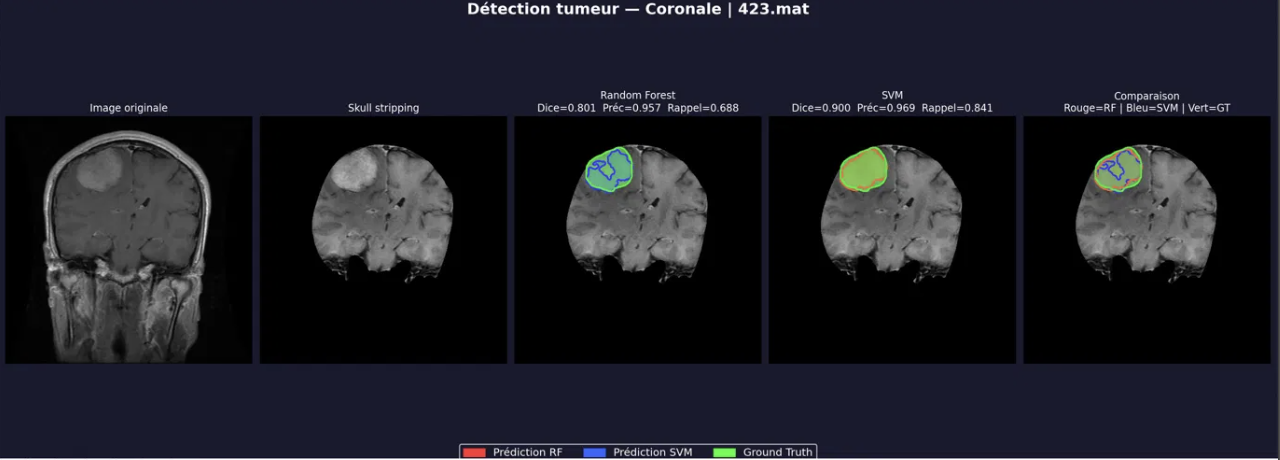
\includegraphics[width=\columnwidth]{423.png}
\caption{Segmentation de 423.mat. De gauche à droite : image 
originale, skull stripping, prédiction RF, prédiction SVM, 
comparaison RF/SVM/GT.}
\label{fig:423}
\end{figure}

\begin{figure}[h]
\centering
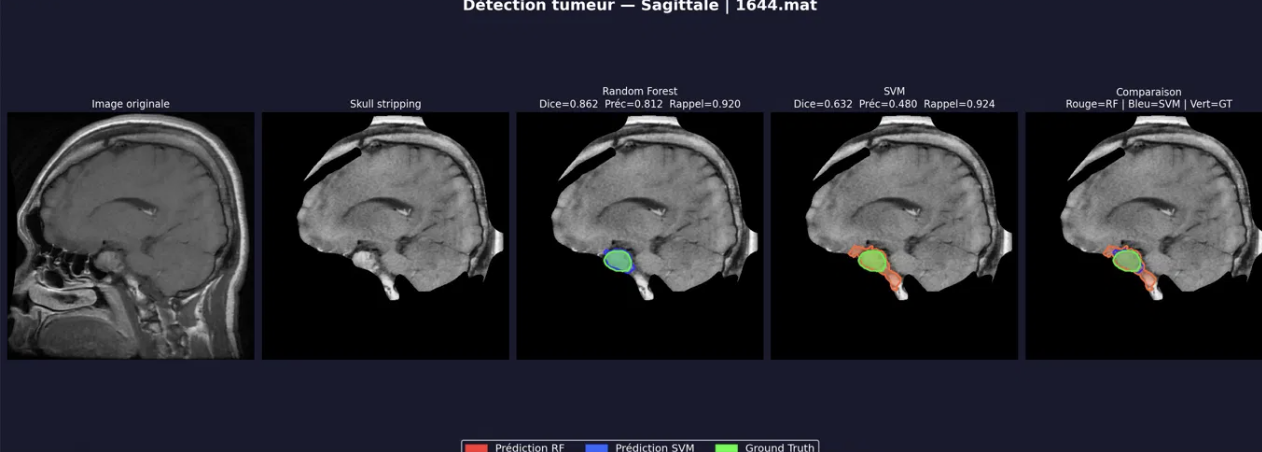
\includegraphics[width=\columnwidth]{1644.png}
\caption{Segmentation de 1644.mat. De gauche à droite : image 
originale, skull stripping, prédiction RF, prédiction SVM, 
comparaison RF/SVM/GT.}
\label{fig:1644}
\end{figure}

\begin{figure}[h]
\centering
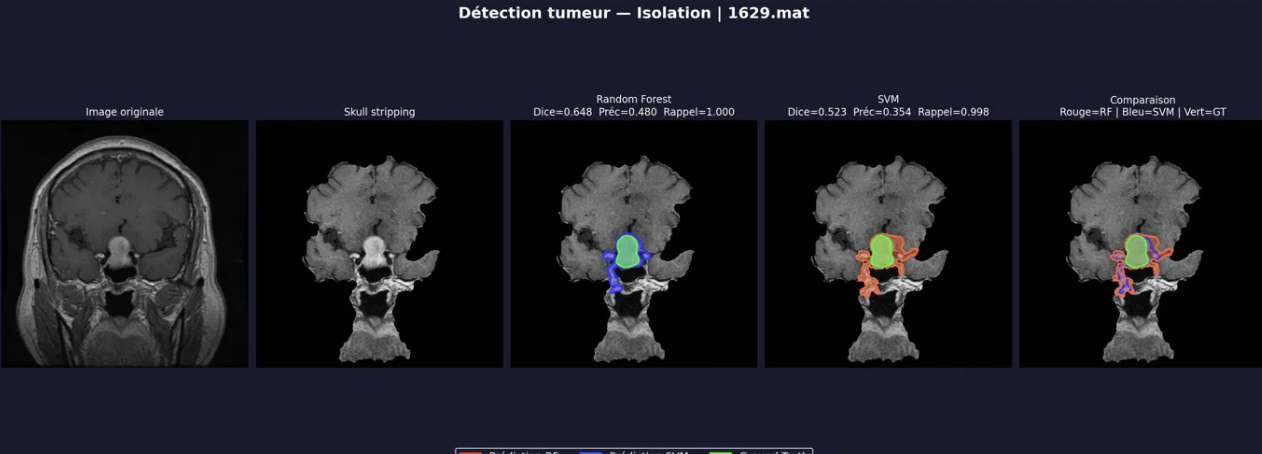
\includegraphics[width=\columnwidth]{1629.png}
\caption{Segmentation de 1629.mat. De gauche à droite : image 
originale, skull stripping, prédiction RF, prédiction SVM, 
comparaison RF/SVM/GT.}
\label{fig:1629}
\end{figure}

\begin{figure}[h]
\centering
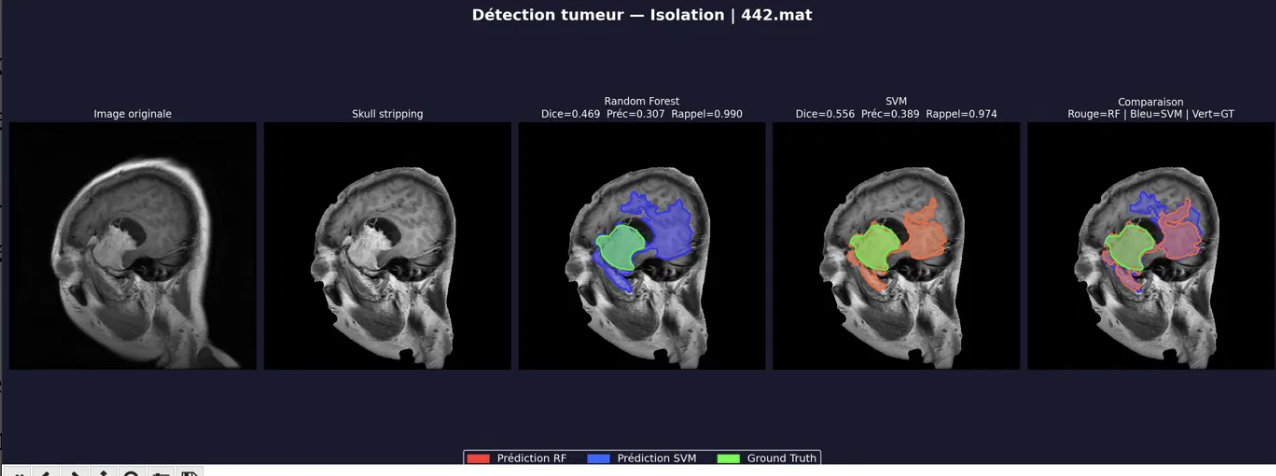
\includegraphics[width=\columnwidth]{442.png}
\caption{Segmentation de 442.mat. De gauche à droite : image 
originale, skull stripping, prédiction RF, prédiction SVM, 
comparaison RF/SVM/GT.}
\label{fig:442}
\end{figure}


\begin{table}[h]
\centering
\caption{Meilleurs résultats obtenus sur les 5 images de test}
\label{tab:resultats}
\begin{tabular}{@{}lccccc@{}}
\toprule
Image & Méthode & Dice RF & Dice SVM & Préc. RF & Rap. RF \\
\midrule
2391.mat & Axiale (m1)   & 0.562 & 0.672 & 0.527 \\
423.mat  & Coronale (m3) & 0.801 & 0.900 & 0.957  \\
1644.mat & Sagittale (m2)& & 0.862 & 0.632 & 0.812 \\
1629.mat & Isolation (m4)& & 0.648 & 0.523 & 0.480 \\
442.mat  & Isolation & 0.469 & 0.556 & 0.307E \\
\midrule
Moyenne  &               & TON\_SCORE & TON\_SCORE & & \\
\bottomrule
\end{tabular}
\end{table}

\subsection{B. Résultats secondaires}
Montrez les résultats secondaires, s’ils existent, et discutez de leur pertinence par rapport à votre objectif. Ce pourrait être des tests supplémentaires, des variations des paramètres ou des résultats obtenus dans différentes conditions.

\section{Discussion et Conclusion}
Dans cette section, fusionnez la discussion et la conclusion. Présentez vos arguments sur la pertinence des méthodes développées et la signification des résultats obtenus.

Discutez des résultats les plus significatifs.

Proposez des explications des phénomènes observés. Pourquoi ces résultats se sont-ils produits ?


Analysez les avantages de votre approche et les limitations possibles. Y a-t-il des biais ou des conditions spécifiques qui ont influencé vos résultats ?

Donnez une perspective d’évolution de vos résultats et des directions futures pour des améliorations.

\section*{Références}
Les références doivent être rédigées selon le format IEEE, comme indiqué ci-dessous. Les références incluent des articles scientifiques, des projets GitHub pertinents, des thèses, et d'autres travaux académiques. Les sources grand public, telles que Wikipédia ou des sites non académiques, ne sont pas acceptées.

\begin{thebibliography}{99}
\bibitem{ref1} Prénom Nom, \textit{Titre de l'article ou du livre}, Journal ou Éditeur, Année.
\bibitem{ref2} Prénom Nom, \textit{Titre du projet Github}, GitHub, URL. Consulté le : Date.
\bibitem{ref3} Prénom Nom, \textit{Titre de la thèse}, Université, Année.
\end{thebibliography}

\end{document}
